\section{Konfigurationstool der 3D-Portfolios (Inhaltserstellung)[L]} \label{Konfigurationstool}
\setauthor{Litzlbauer Lorenz}

Die Inhaltserstellung-Funktion war eine der Kernfunktionen des Projekts. Mit die Inhaltserstellung konnten die 3D-Portfolios erst entstehen. Es galt einen einfachen und intuitiven Konfigurationsprozess für 3D-Portfolios zu gestalten. Im Entwicklungsprozess wurden viele Entscheidungen getroffen, die auf das ganze Projekt Einfluss hatten. Z.B. wurde eine Art der Datenrepräsentation der 3D-Portfolios und die Darstellungsweise der Daten in der 3D-View entwickelt.

In diesem Kapitel wird die Entwicklung und das System der Inhaltserstellung erklärt.

\begin{figure}
    \centering
    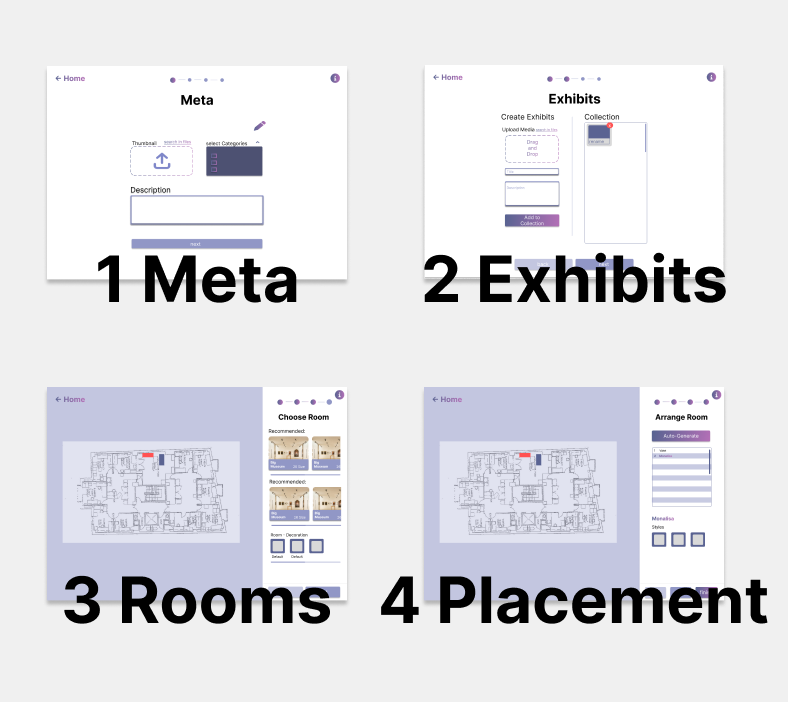
\includegraphics[scale=0.5]{pics/CreateCreation4Categories.png}
    \caption{Die vier Erstellungskategorien}
    \label{fig:impl:creation:fourCategoires}
\end{figure}

\subsection{Überblick [L]}
Das Inhaltserstellung-Tool besteht aus insgesamt vier Unterseiten (siehe Abbildung \ref{fig:impl:creation:fourCategoires}), mit diesen werden Daten gesammelt, um das Portfolio zu erstellen und vielen Untersystemen (bestehend aus Komponenten, Klassen und Services siehe Unterkapitel \ref{sec::impl::contentcreation::UnterstuetzendeServicesUndKlassen} auf Seite \pageref{sec::impl::contentcreation::UnterstuetzendeServicesUndKlassen}) , die beim Erstellungsprozess helfen.

Diese Unterseiten wurden aufgeteilt, damit der*die Benutzer*in sich im Konfigurationsprozess nur mit jeweils einer Portfolio-Daten-Kategorie beschäftigen muss und nicht überfordert wird. Dabei wurde sich  am \emph{Wizard-UI-Pattern} (mehr dazu im Unterkapitel \ref{sec::contentcreation::wizard} auf der Seite \pageref{sec::contentcreation::wizard}) orientiert.

\subsection{Userinterface-Struktur / Wizard Design Pattern [L]}
\label{sec::contentcreation::wizard}
Im Projekt wurde das Wizard-UI-Pattern benutzt, um den Konfigurationsprozess des Portfolios einfacher zu gestalten. Dafür wurden die Konfigurationsdaten nach 4 Kategorien aufgeteilt und für jede eine eigene Unterseite (siehe Abbildung \ref{fig:impl:creation:fourCategoires}) entworfen.

Die Kategorien sind:
\begin{compactitem}
\item Metadaten - Die Metadaten sind Daten, die das Portfolio beschreiben, dazu gehören Name, zugehörige Kategorien, eine Beschreibung und ein Thumbnail.
\item Ausstellungsstück - Die Daten des Ausstellungsstücks bestehen aus den vom User auf den Server geladenen Kunstwerken und Zusatzinformation wie Namen und Beschreibung.
\item Raumdaten - Raumdaten bestehen aus den virtuellen 3D-Daten des Raumes und weiteren Konfigurationsdaten wie den Positionen, an denen Ausstellungsstücke im Raum platziert werden können.
\item Ausstellungsplatzierungsdaten - Mit diesen Daten werden die Daten zu den Ausstellungsstücken und dem virtuellen Raum logisch verbunden.
\end{compactitem}

\subsubsection*{Begriffserklärung [L]}
Der Begriff "\emph{Wizard}" in der Softwareentwicklung, kommt ursprünglich von Systemadministratoren, welche bei komplizierten Installationsprozessen halfen oder ganz übernahmen. Mit der Zeit änderte sich der Begriff zu Software-Assistenten-Programmen, welche dem*der User*in dabei unterstützten, die Software zu konfigurieren. \cite[Ursprung des Begriffs Wizard]{OrigionOfWizards}

\subsubsection{Wizard-UI-Pattern [L]}
Im Web-Bereich gibt es in der Regel zwei Arten Dateneintragungen zu verarbeiten.

Formulare und Wizards. Virtuelle Formulare sind dabei ähnlich aufgebaut wie reale Formulare, in denen die Formularfelder ausgeführt werden sollen. Hingegen ist ein Wizard eine eigene kleine Applikation, die den*die Benutzer*in durch eine Folge von Formularen führt und gegebenenfalls beim Ausfüllen unterstützt. Je nach den Eingaben können Wizards die Reihenfolge oder die Formulare ändern.

TODO: Bei Bedarf könnte hier mehr geschrieben werden. \cite[Wizards: Definition and Design Recommendations]{WizradsDefinitionAndRecommandation}

\subsubsection{Implementation [L]}
Für die Implementation des Wizards wurde die Angular Material Komponente Mat-Stepper benutzt. Sie bietet eine solide Basis für den Wizard. Content kann sequentiell dargestellt werden, während dem*der User*in der aktuelle Status des Wizards durch eine Navigationsleiste angezeigt wird (siehe Abbildung \ref{fig:impl:creation:mathorziontalstepper}). \cite{amStepper}

\begin{figure}
    \centering
    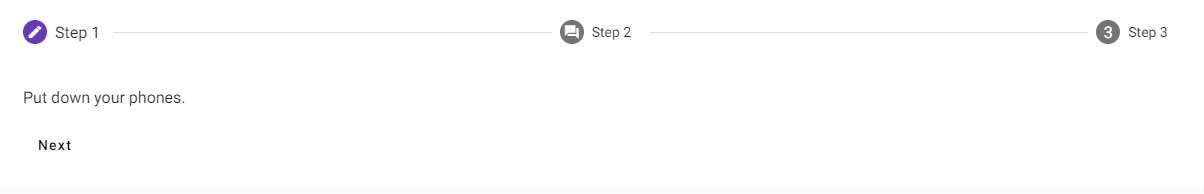
\includegraphics[scale=0.5]{pics/mathorziontalstepper.png}
    \caption{Angular Material: horizontaler Stepper \cite{amStepper}}
    \label{fig:impl:creation:mathorziontalstepper}
\end{figure}

\subsection{4 Formularunterseiten [L]}
Nachdem die Angular Material Komponente Mat-Stepper für die Wizard-Funktionalität gewählt wurde, war der nächste Schritt, die vier Formularunterseiten des Wizards (siehe Abbildung \ref{fig:impl:creation:fourCategoires}) zu gestalten.

In diesem Unterkapitel werden die Funktionalitäten und die Probleme bzw. Lösungen dieser Unterseiten beschrieben. 

\subsubsection{Kommunikationsschnittstelle [L]}
Die Unterseiten sammeln Daten für die Erstellung des Portfolios. Die Kommunikationsschnittstellen der Unterseiten helfen dabei, dass die Unterseiten miteinander kommunizieren können. Dafür wurde das \emph{Observer-Design-Pattern} (siehe im Glossar \ref{txt:glos:observerDesignPattern} auf Seite \pageref{txt:glos:observerDesignPattern}) gewählt.

In einer Dienstklasse, die durch Dependency Injection (siehe Unterkapitel \ref{DPI} auf Seite \pageref{DPI}) mit allen Unterseiten verbunden ist, befinden sich Observablen, die mit den Eingabefeldern der Unterseiten verbunden sind. Wenn auf den Unterseiten eine neue Dateneingabe geschieht, wird die Veränderung an die Dienstklasse weitergegeben. Die Unterseiten haben jeweils eine Datenklasse nach den Kategorien des Portfolios (siehe Abbildung \ref{fig:impl:creation:dataclasses}), in der die Daten gespeichert werden.

\begin{figure}
    \centering
    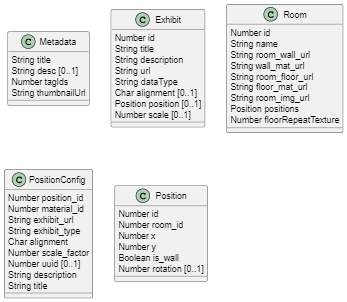
\includegraphics[scale=0.7]{pics/content_creation_classes.png}
    \caption{Inhaltserstellung Datenklassen}
    \label{fig:impl:creation:dataclasses}
\end{figure}

In der Dienstklasse werden Veränderungen durch den SessionStorage (siehe Unterkapitel \ref{par:impl:usermanagment:WebStorage} auf Seite \pageref{par:impl:usermanagment:WebStorage}) gespeichert und an den Wizard Mat-Stepper weitergeleitet, um dort den Fortschritt des Konfigurationsprozesses anzuzeigen.

Durch die Speicherung im SessionStorage kann der Konfigurationsprozess selbst bei einem Abbruch in der Zukunft nahtlos fortgesetzt werden.

\subsubsection{Metadaten - Unterseite [L]}
Die Metadaten-Unterseite (siehe Abbildung \ref{fig:impl:creation:Metadaten_Unterseite}) wurde erstellt, um Metadaten wie den Namen, die Kategorien, das Vorschaubild und eine kurze Beschreibung zu der Ausstellung zu sammeln.

Alphanumerische Daten wie der Name und die Beschreibung wurden mit Angular's reaktiven Formularen (siehe Kapitel \ref{par:impl:usermanagment:reactiveForms} auf Seite \pageref{par:impl:usermanagment:reactiveForms}) gesammelt.

Das Vorschaubild wird hochgeladen mit der Dateien-Hochlade-Komponente (siehe Kapitel \ref{sec:impl:contentcreation:file-Upload} auf Seite \pageref{sec:impl:contentcreation:file-Upload}). Auf der Webapplikation wird die URL gespeichert, unter der die hochgeladene Datei zur Verfügung steht.

\begin{figure}
    \centering
    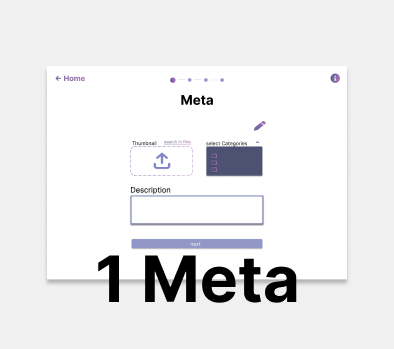
\includegraphics[scale=0.5]{pics/metadaten.png}
    \caption{Metadaten Unterseite}
    \label{fig:impl:creation:Metadaten_Unterseite}
\end{figure}

\subsubsection{Ausstelungsstücke - Raum}
\subsection{Unterstützende Services und Klassen}
\label{sec::impl::contentcreation::UnterstuetzendeServicesUndKlassen}
\subsubsection{Dateien-Hochlade-Komponente [L]}
\label{sec:impl:contentcreation:file-Upload}

TODO: Image vom der Komponente

Die Dateien-Hochlade-Komponente wurde mit dem Gedanken entwickelt, hoch modular und anpassungsfähig zu sein. Denn die Hochlade-Funktion wird öfters im Projekt gebraucht.

Bei der Komponente sind akzeptable Filetypen und Filegrößen einzustellen, werden die gesetzten Anforderungen an Filetypen und Filegrößen von den hochzuladenden Daten nicht erfüllt, so werden diese auch nicht hochgeladen und die Komponente gibt eine Fehlermeldung.
Bei einem erfolgreichen Hochladeprozess bekommt die Komponente eine URL vom Server. Unter der URL ist die hochgeladene Datei erreichbar.

\paragraph{Funktionalitäten und Implementierung [L]}
\paragraph{Hochlade Funktionalitäten des Servers [E]}


\subsubsection{Portfolio-Veröffentlichung-System [L]}